%
% 注意 EWinTeX3 では，TeXを掛ける　T　ボタンの後，
% 外部アプリ中の「1 dvi > PDF (sample)」を 呼び出す．　TP　ボタンは使わない．
% プレビューは，dvioutや Acrobat や Edge を使わずに，SumatoraPDF を用いる．
%
\documentclass[dvipdfmx,12pt,aspectratio=169]{beamer}
%aspectratioは横縦比16:9，1610とすれば16:10に．省けば4:3に．
%ノートPCの画面サイズを調べて、合わせましょう．
%フォントサイズは11pt,12ptなどもありますが，12ptか14ptが良いでしょう
\usepackage{graphicx}
\usepackage{xcolor} %tcolorboxで色を変えたから
\usepackage{bxdpx-beamer}% dvipdfmxなので必要
\usepackage{pxjahyper}% 日本語で'しおり'したい
\usepackage{minijs}% min10ヤダ
\renewcommand{\kanjifamilydefault}{\gtdefault}% 既定をゴシック体に

\usetheme{Boadilla}
%themeは https://tex.y-misc.org/beamer/theme.html を参照
\setbeamercovered{transparent}%消えている文字をうっすらと表示する
\usepackage{tcolorbox} %色を変えたboxを使うなら．

\usepackage{amsmath} %align環境などの数式環境に
\usepackage{amssymb} %特殊な数式シンボルに必須
\usepackage{amsthm} %theorem環境に．
%上の３つは{amsmath,amssymb,amsthm}とまとめても．
\renewcommand\proofname{\bf 証明} %Proofではなく証明


\usepackage{tikz}%お絵描きするなら必要
\usetikzlibrary{calc, intersections, through, backgrounds} % tikzの拡張ライブラリ


\theoremstyle{definition} %見出しは太字，本文で斜体を使わない
\newtheorem{dfn}{定義}
\newtheorem{thm}[dfn]{定理}
\newtheorem{prp}[dfn]{命題}
\newtheorem{lmm}[dfn]{補題}


\definecolor{forestgreen}{rgb}{0.13, 0.55, 0.13}
%forestgreen色を使いたかった

%%%%%%%%%%%%%%%%%%%%%%%%%%%%%%%%%%%%%%%%%%%%%%%%%%%%%%%%%%%%%
%%%%%%%%%%%%%%%%%%%%%%%プリアンブル終り%%%%%%%%%%%%%%%%%%%%%%
%%%%%%%%%%%%%%%%%%%%%%%%%%%%%%%%%%%%%%%%%%%%%%%%%%%%%%%%%%%%%
\title{微分を使わない極値・最小値探索手法}
\subtitle{Brent法のアルゴリズムと数学的性質}
\author{imohiyoko}
\date{2026年 02月 12 日(木)}


\begin{document}

% =========================================================
% タイトルページ
% =========================================================
\maketitle

% =========================================================
% 目次
% =========================================================
\begin{frame}
 \frametitle{本発表の流れ}
 \tableofcontents
\end{frame}

% =========================================================
% 各章の読み込み
% =========================================================
\begin{frame}
 \frametitle{発表の背景}
    数値計算において、関数の最大、最小値をより高精度な値で求めたいという要件が発生することがある。
    その時、微分などを用いて探索を行うのは困難な場合がよくおこるあ。
    そこで、微分情報を用いずに関数の極値を効率的に探索する手法があると嬉しい。
\end{frame}
\begin{frame}
    実際、私の卒業研究のRemesアルゴリズムによる最良近似多項式の計算においても、極値探索が必要となりました。
    はじめは放物線近似を使えばある程度うまくいきそうだと考えて調べると、Brent法という非常に有名な手法があることがを発見した。
    ここではなんか研究過程でたどり着いたBrent法というものが面白かったのでそのアルゴリズムとその歴史について紹介します。
\end{frame} % はじめに
\section{黄金分割法}

%-----------------------------------------------------------
% 1. 黄金分割法
%-----------------------------------------------------------
\begin{frame}
    \frametitle{黄金分割法の歴史}
    黄金分割法の原理に基づく探索手順は、1953年にKieferの論文「Sequential Minimax Search for a Maximum」の中で提案されました。
    この論文の主題は観測回数が固定されたときフィボナッチ数を用いた探索法でしたが、
    黄金分割法も同時に紹介されました。
\end{frame}

% このファイルは自動生成されました
% 親ファイル(tex_soturonhappyoルート)から \input して使用することを想定しています

% フレーム1: フィボナッチ法（補足1）
\begin{frame}
  \frametitle{フィボナッチ法による最適探索}
  \begin{columns}
    \begin{column}{0.45\textwidth}
      \small
      \textbf{補足：} Kiefer氏は観測回数が固定された場合、フィボナッチ数を用いた探索法を提示しました。
      
      \vspace{0.5em}
      \begin{itemize}
        \item 観測回数が\textbf{事前に決定}されている
        \item フィボナッチ数により最悪ケースを最適化
        \item 関数値が小さい側に拡大
        \item 赤点：新規評価点
      \end{itemize}
      
      \vspace{0.5em}
      \textbf{目的関数:} $f(x) = (x-2)^2 + 0.5\sin(3x)$
    \end{column}
    \begin{column}{0.55\textwidth}
      \centering
      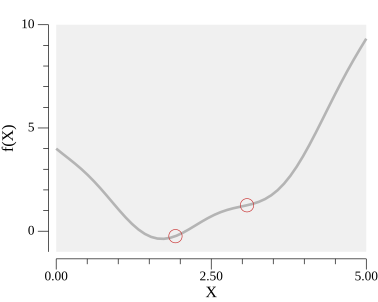
\includegraphics[width=\textwidth]{material/kiefer/output/fibonacci_fixed_obs.png}
    \end{column}
  \end{columns}
\end{frame}

% フレーム2: 黄金比を用いた方法（補足2）
\begin{frame}
  \frametitle{黄金比を用いたアルゴリズム}
  \begin{columns}
    \begin{column}{0.45\textwidth}
      \small
      \textbf{補足：} これとは別に、黄金比を用いて常に同じアルゴリズムで区間を縮小する手順が提示されました。
      
      \vspace{0.5em}
      \begin{itemize}
        \item 黄金比 $\phi = \frac{\sqrt{5}-1}{2} \approx 0.618$
        \item \textbf{同じアルゴリズム}を繰り返す
        \item 観測回数は事前に決めない
        \item 関数が単峰性を保つ限り有効
      \end{itemize}
      
      \vspace{0.5em}
      これが一般に\textbf{黄金分割法}と呼ばれます。
    \end{column}
    \begin{column}{0.55\textwidth}
      \centering
      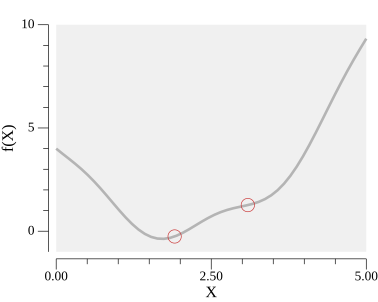
\includegraphics[width=\textwidth]{material/kiefer/output/golden_ratio_method.png}
    \end{column}
  \end{columns}
\end{frame}

% フレーム3: 黄金分割法の実用性（補足3）
\begin{frame}
  \frametitle{黄金分割法の実用性}
  \begin{columns}
    \begin{column}{0.45\textwidth}
      \small
      \textbf{補足：} 黄金分割法は厳密には最適な手順ではありませんが、観測回数を事前に決めない場合に特に有用です。
      
      \vspace{0.5em}
      \begin{itemize}
        \item 各段階で区間は最悪でも $0.618$ 倍に縮小する
        \item 実装が簡単で安定している
        \item 収束性が良好
        \item 観測回数を任意に変更可能
      \end{itemize}
      
      \vspace{0.5em}
      \textbf{利点:} 実用性と安定性のバランスが優れている
    \end{column}
    \begin{column}{0.55\textwidth}
      \centering
      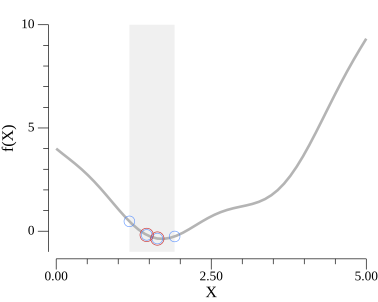
\includegraphics[width=\textwidth]{material/kiefer/output/golden_section_no_fixed_obs.png}
    \end{column}
  \end{columns}
\end{frame}





% このファイルは自動生成されました。
% 親ファイル(tex_soturonhappyoルート)から \input して使用することを想定しています。
\begin{frame}{黄金分割法の収束プロセス}
  \begin{columns}
    \begin{column}{0.4\textwidth}
      \begin{itemize}
        \item \textbf{グレー領域}: 現在の探索区間
        \item \textcolor{red}{\textbf{赤丸}}: 今回の評価点
        \item \textcolor{blue}{\textbf{青丸}}: 既存の評価点
      \end{itemize}
      \vspace{1em}
      範囲が狭まるにつれ、範囲外の点は探索対象から除外（消去）されます。
    \end{column}
    \begin{column}{0.6\textwidth}
      \centering
      \only<1>{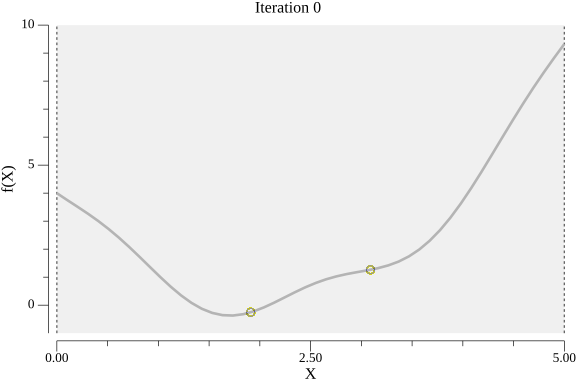
\includegraphics[width=\textwidth]{material/golden/output/golden_00.png}}
      \only<2>{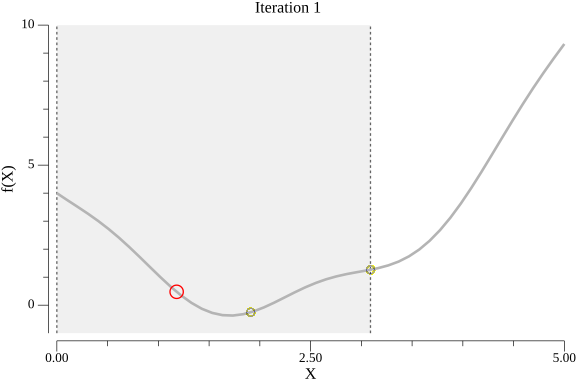
\includegraphics[width=\textwidth]{material/golden/output/golden_01.png}}
      \only<3>{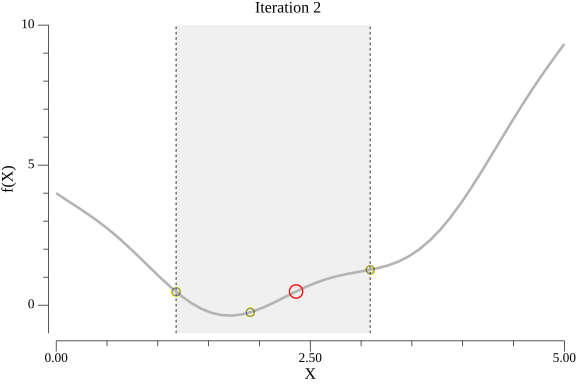
\includegraphics[width=\textwidth]{material/golden/output/golden_02.png}}
      \only<4>{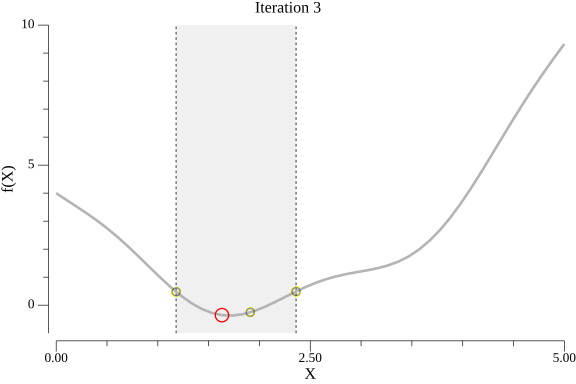
\includegraphics[width=\textwidth]{material/golden/output/golden_03.png}}
      \only<5>{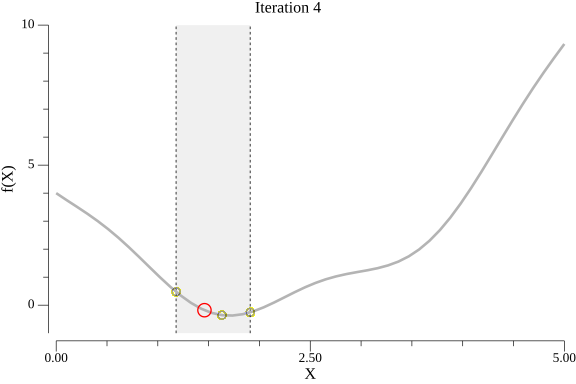
\includegraphics[width=\textwidth]{material/golden/output/golden_04.png}}
      \only<6>{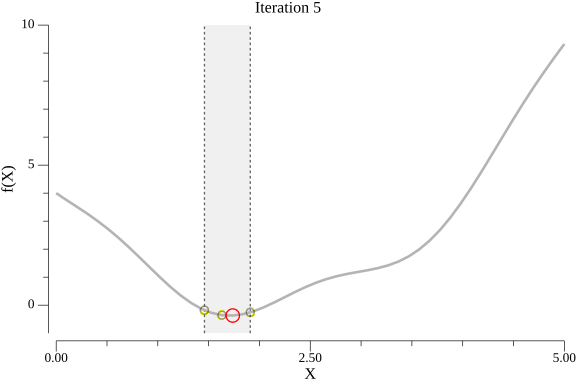
\includegraphics[width=\textwidth]{material/golden/output/golden_05.png}}
      \only<7>{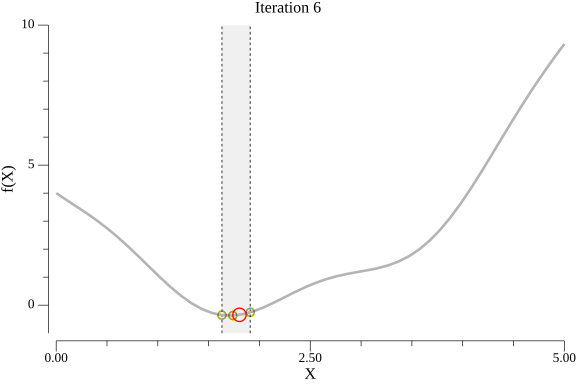
\includegraphics[width=\textwidth]{material/golden/output/golden_06.png}}
      \only<8>{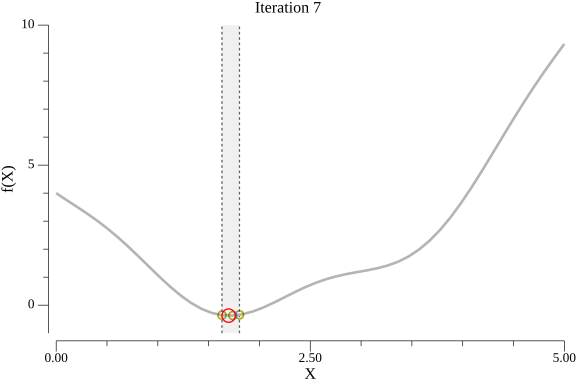
\includegraphics[width=\textwidth]{material/golden/output/golden_07.png}}
      \only<9>{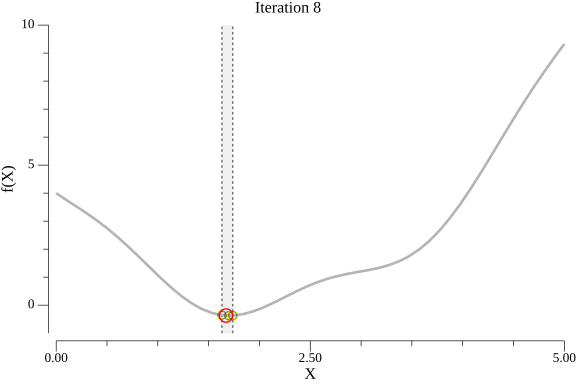
\includegraphics[width=\textwidth]{material/golden/output/golden_08.png}}
      \only<10>{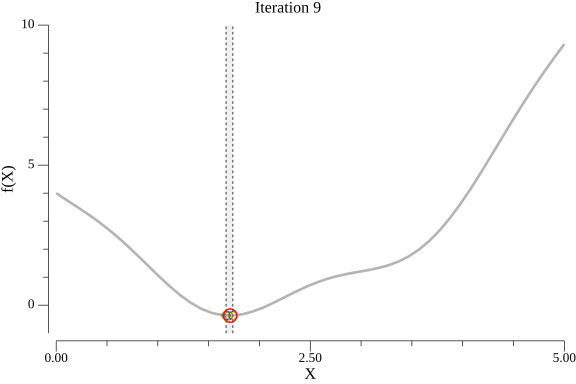
\includegraphics[width=\textwidth]{material/golden/output/golden_09.png}}
      \only<11>{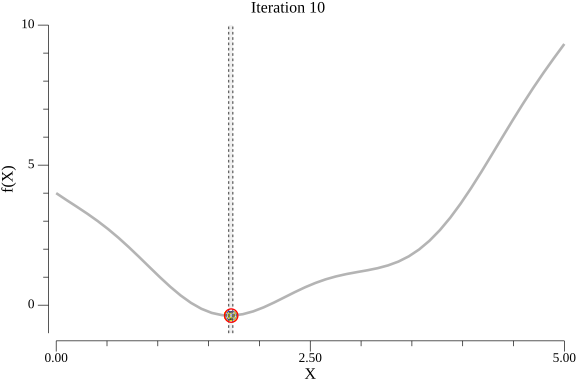
\includegraphics[width=\textwidth]{material/golden/output/golden_10.png}}
      \only<12>{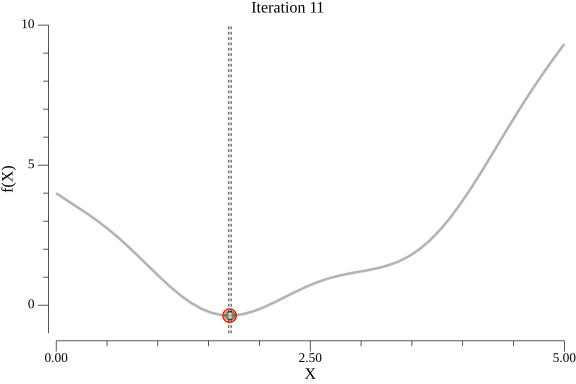
\includegraphics[width=\textwidth]{material/golden/output/golden_11.png}}
      \only<13>{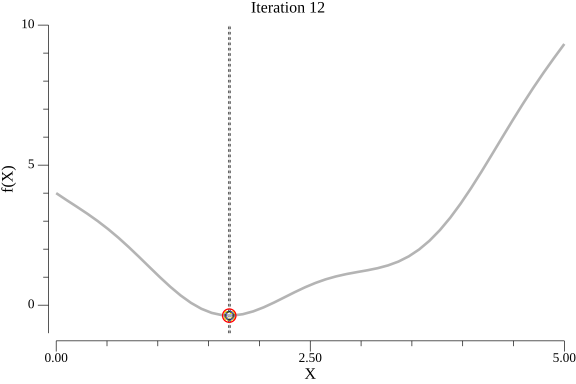
\includegraphics[width=\textwidth]{material/golden/output/golden_12.png}}
      \only<14>{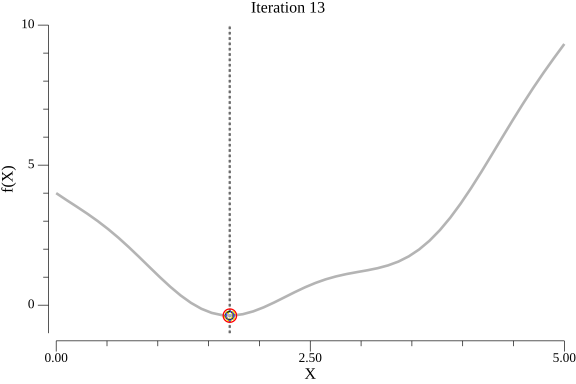
\includegraphics[width=\textwidth]{material/golden/output/golden_13.png}}
      \only<15>{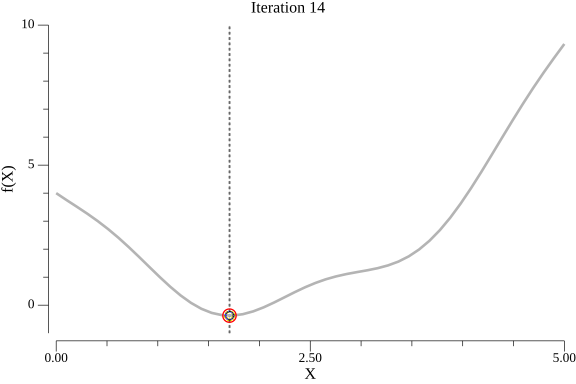
\includegraphics[width=\textwidth]{material/golden/output/golden_14.png}}
      \only<16>{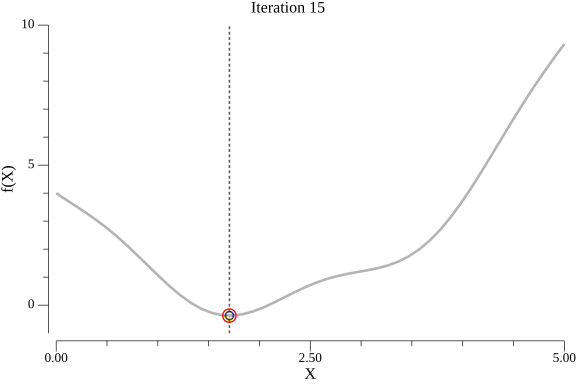
\includegraphics[width=\textwidth]{material/golden/output/golden_15.png}}
    \end{column}
  \end{columns}
\end{frame}


\begin{frame}
\frametitle{黄金分割法の収束性}
\section*{1. 新しい点の位置関係の定義}
極小を囲う3点 $a < b < c$ について、比率 $W$ と $Z$ を定義します。
\begin{itemize}
    \item $W = \frac{b-a}{c-a}$
    \item $1-W = \frac{c-b}{c-a}$
\end{itemize}

\centering
\vspace{0.2cm}
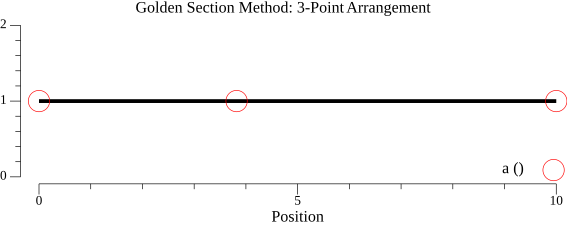
\includegraphics[width=0.7\textwidth]{material/convergence/output/diagram1_points.png}
\end{frame}

\begin{frame}
\frametitle{黄金分割比の導出（2）}
\section*{2. 最悪ケースの縮小率最適化}
新しい点 $x$ の位置を、最悪ケースの縮小率を最適化するために決定します：
\begin{itemize}
    \item 条件: $ W+Z = 1-W $
    \item 導出: $ Z = 1 - 2W $
\end{itemize}

\centering
\vspace{0.2cm}
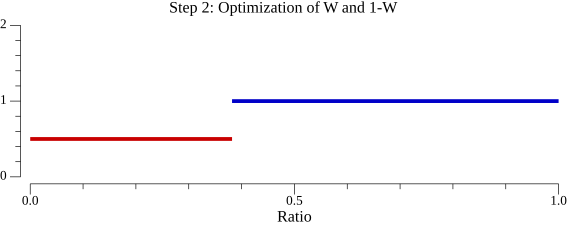
\includegraphics[width=0.7\textwidth]{material/convergence/output/diagram2_optimization.png}
\end{frame}

\begin{frame}
\frametitle{黄金分割比の導出（3）}
\section*{3. スケール相似性}
新しい区間でも同じ比率を保つという相似性の原理：
\begin{itemize}
    \item 相似条件: $ \frac{Z}{1-W} = W $
    \item 新区間と元区間の比率が常に等しい
\end{itemize}

\centering
\vspace{0.2cm}
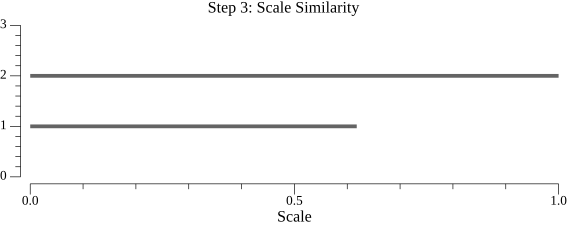
\includegraphics[width=0.7\textwidth]{material/convergence/output/diagram3_similarity.png}
\end{frame}

\begin{frame}
\frametitle{黄金分割比の導出（4）・収束性}
\section*{4. 黄金分割比と収束率}
比率条件より、以下の方程式を得ます：
\begin{itemize}
    \item 二次方程式: $ W^2 - 3W + 1 = 0 $
    \item 解: $ W = \frac{3 - \sqrt{5}}{2} \approx 0.38197 $
    \item 黄金比: $ \phi = \frac{\sqrt{5}-1}{2} \approx 0.618 $
    \item 収束率: 各ステップで区間は $\phi$ 倍に縮小（1次収束）
\end{itemize}

\centering
\vspace{0.2cm}
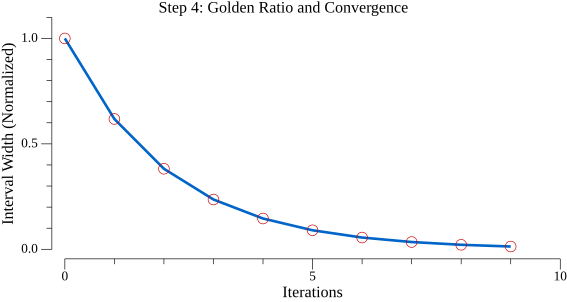
\includegraphics[width=0.7\textwidth]{material/convergence/output/diagram4_convergence.png}
\end{frame}
 % 黄金分割法の歴史と収束速度の証明
\section{放物線補間法}


% 放物線補間 (SPI) のアニメーション
\begin{frame}{放物線補間の収束プロセス}
  \begin{columns}
    \begin{column}{0.4\textwidth}
      \begin{itemize}
        \item \textcolor{blue}{\textbf{青丸}}: 補間に使用する3点
        \item \textcolor{green}{\textbf{緑破線}}: 3点を通る近似放物線
        \item \textcolor{red}{\textbf{赤丸}}: 放物線の頂点 
      \end{itemize}
      \vspace{1em}
      \small
      頂点付近では極めて高速に収束するが、初期値が悪いと放物線が反転して遠くへ飛んだり、更新が停滞したりするリスクがある。
    \end{column}
    \begin{column}{0.6\textwidth}
      \centering
      \only<1>{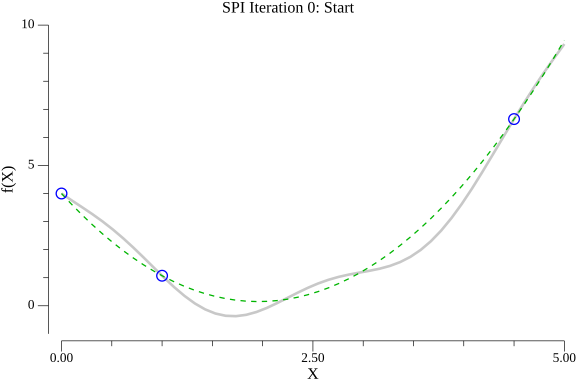
\includegraphics[width=\textwidth]{material/spi/output/spi_00.png}}
      \only<2>{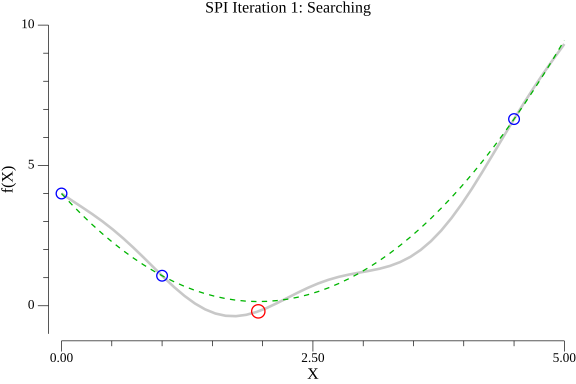
\includegraphics[width=\textwidth]{material/spi/output/spi_01.png}}
      \only<3>{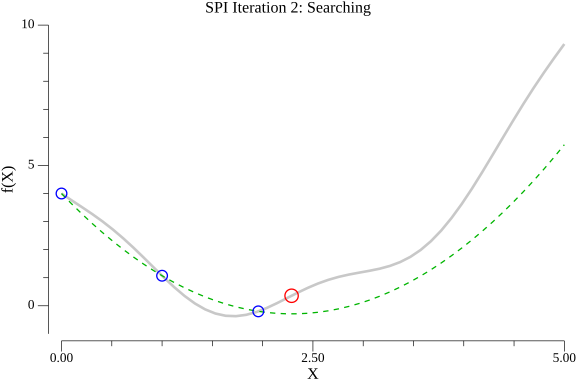
\includegraphics[width=\textwidth]{material/spi/output/spi_02.png}}
      \only<4>{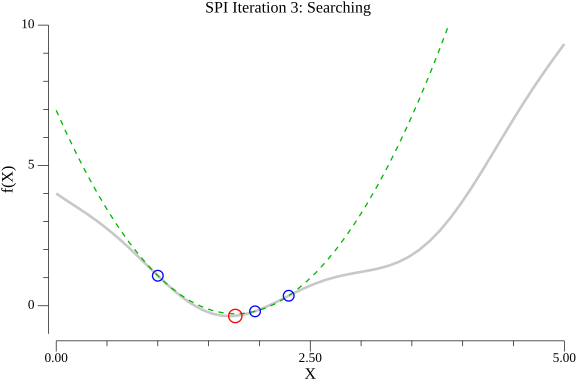
\includegraphics[width=\textwidth]{material/spi/output/spi_03.png}}
      \only<5>{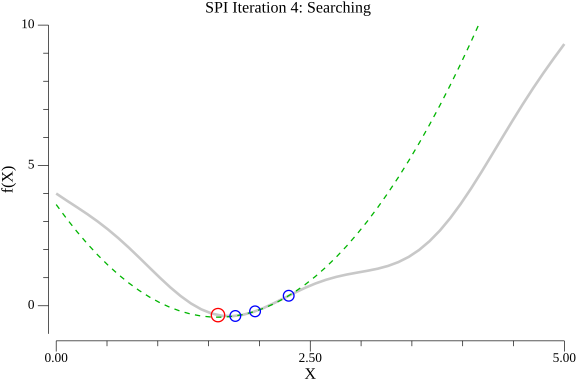
\includegraphics[width=\textwidth]{material/spi/output/spi_04.png}}
      \only<6>{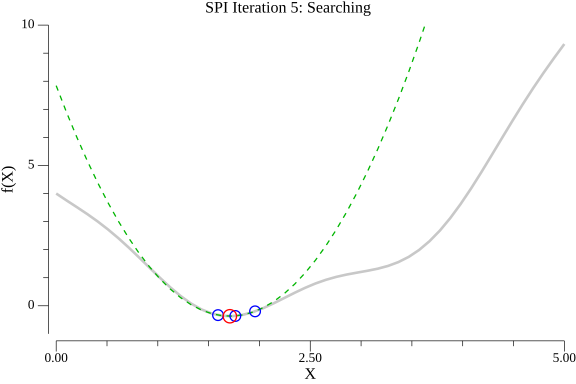
\includegraphics[width=\textwidth]{material/spi/output/spi_05.png}}
      \only<7>{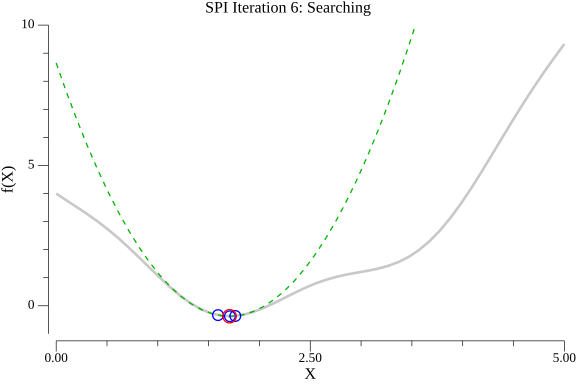
\includegraphics[width=\textwidth]{material/spi/output/spi_06.png}}
      \only<8>{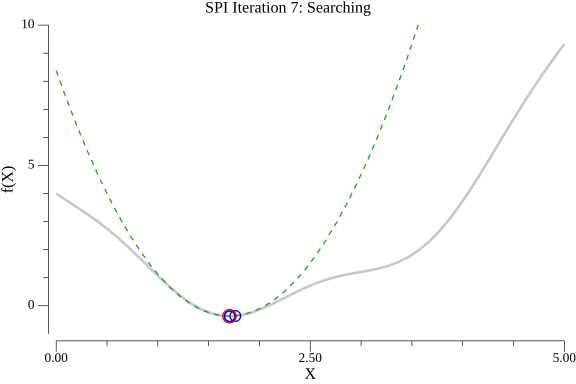
\includegraphics[width=\textwidth]{material/spi/output/spi_07.png}}
      \only<9>{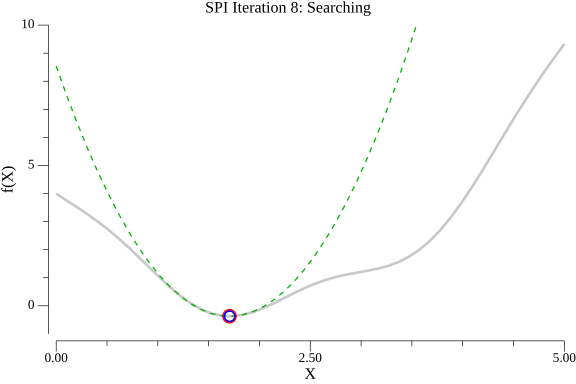
\includegraphics[width=\textwidth]{material/spi/output/spi_08.png}}
      \only<10>{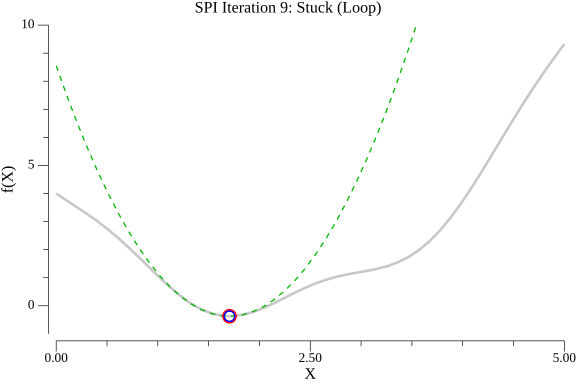
\includegraphics[width=\textwidth]{material/spi/output/spi_09.png}}
    \end{column}
  \end{columns}
\end{frame}

 % 放物線補間法のアルゴリズムと不安定さを示す
%===========================================================
% 3. Brent法
%===========================================================
\section{黄金分割法と放物線補間の融合}

\begin{frame}
 \frametitle{Brent法のコンセプト}
 
 \textbf{基本的な考え方:}
  各反復で「どちらの戦略を使うか」を判定
  \begin{itemize}
   \item 放物線補間が信頼できそう $\Rightarrow$ 使う
   \item そうでない $\Rightarrow$ 黄金分割に切り替え
 \end{itemize}
\end{frame}
\begin{frame}
  常に3つの良い候補点 $(x, w, v)$ と 極値が必ず存在する区間 $[a^*, b^*]$ を保持
  \begin{itemize}
   \item $x$：現在の最良点（最も良い関数値）
   \item $w$：2番目に良い点
   \item $v$：3番目に良い点（または直前の$w$）
   \item $a^*$：極値が存在する区間の左端点 
   \item $b^*$：極値が存在する区間の右端点
  \end{itemize}
  
  条件によって二つの手法を取る
  \begin{itemize}
   \item  $x,w,v$ を用いて放物線補間で次の点を探す
   \item  $a^*,x ,b^*$ と黄金分割で堅実さを保証
  \end{itemize}
\end{frame}

\begin{frame}
 \frametitle{Brent法：強制二分条件}

 \textbf{放物線補間を採用するための判断条件:}
 前々回の$x$から試みた移動距離 $e$、今回の放物線補間による軸と現在の$x$との距離を $d$ とするとき、
 以下を満たさなければならない：
 
 \begin{tcolorbox}[colback=red!10!white, colframe=red!75!black, title=強制二分条件]
  \begin{equation*}
   |d| < \frac{1}{2}|e|
  \end{equation*}
 \end{tcolorbox}
\end{frame}

%% Brent法の収束過程のグラフをここに貼る

% Brent法のアニメーション
\begin{frame}{Brent法：ハイブリッド戦略の可視化}
  \begin{columns}
    \begin{column}{0.4\textwidth}
      \begin{itemize}
        \item \textbf{グレー領域}: 解を囲む区間 $[a, b]$
        \item \textcolor{blue}{\textbf{青丸}}: 現在の主要な3点 ($x, w, v$)
        \item \textcolor{red}{\textbf{赤丸}}: 今回の試行点 $u$
        \item \textcolor{green}{\textbf{緑破線}}: 採用された近似放物線
      \end{itemize}
      \vspace{1em}
      \small
      基本は放物線補間を試み、条件が悪い場合（緑線が出ない回）は安全な黄金分割を選択している様子がわかる。
    \end{column}
    \begin{column}{0.6\textwidth}
      \centering
      \only<1>{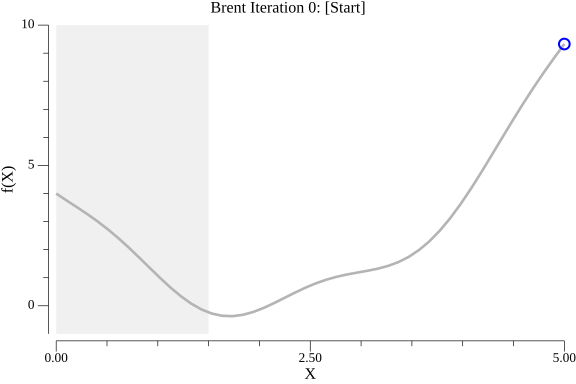
\includegraphics[width=\textwidth]{material/brent/output/brent_00.png}}
      \only<2>{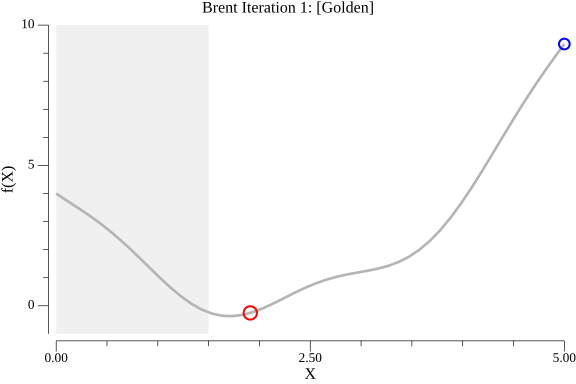
\includegraphics[width=\textwidth]{material/brent/output/brent_01.png}}
      \only<3>{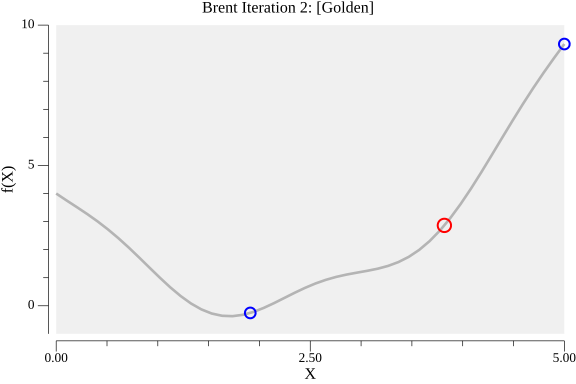
\includegraphics[width=\textwidth]{material/brent/output/brent_02.png}}
      \only<4>{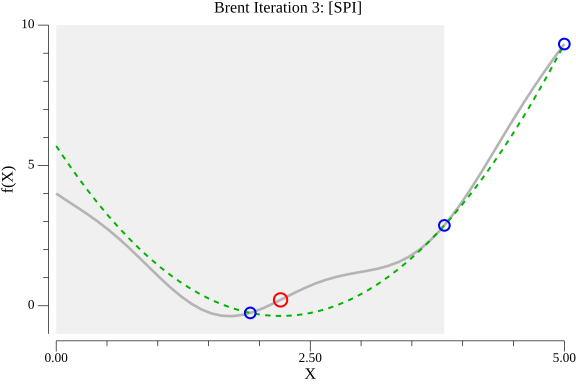
\includegraphics[width=\textwidth]{material/brent/output/brent_03.png}}
      \only<5>{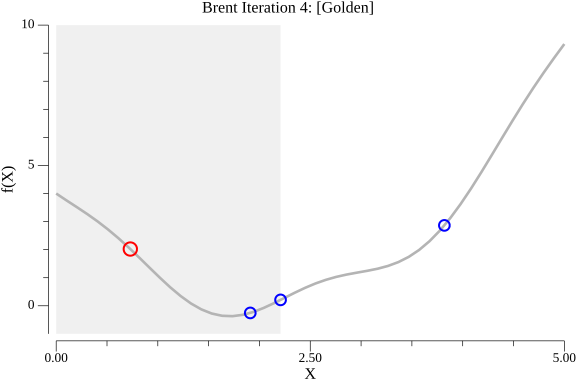
\includegraphics[width=\textwidth]{material/brent/output/brent_04.png}}
      \only<6>{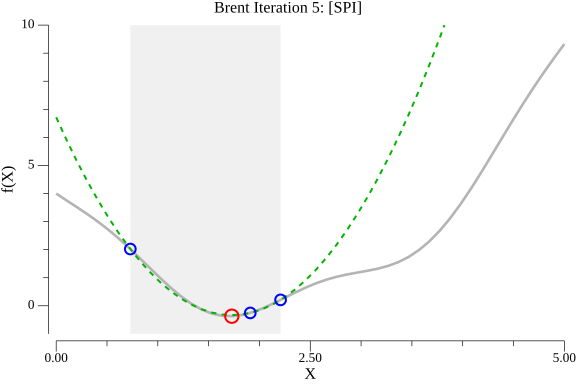
\includegraphics[width=\textwidth]{material/brent/output/brent_05.png}}
      \only<7>{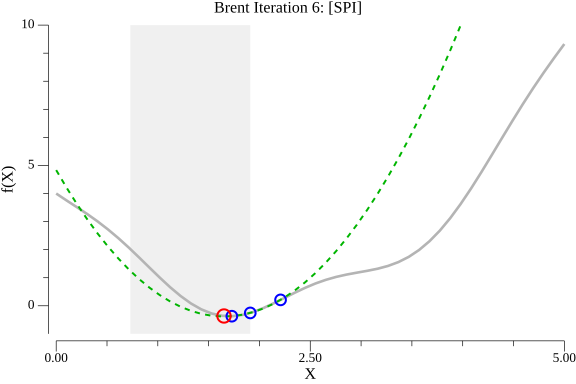
\includegraphics[width=\textwidth]{material/brent/output/brent_06.png}}
      \only<8>{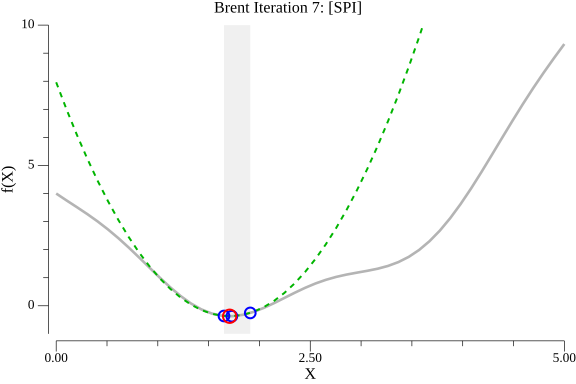
\includegraphics[width=\textwidth]{material/brent/output/brent_07.png}}
      \only<9>{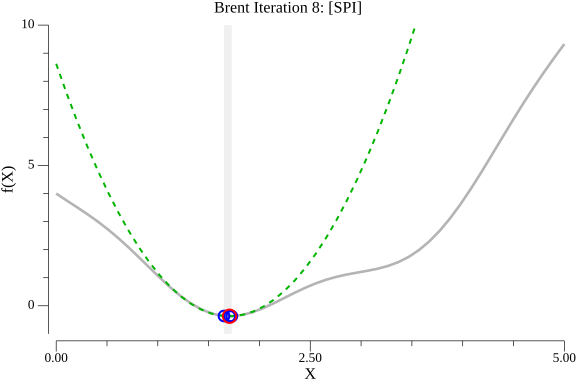
\includegraphics[width=\textwidth]{material/brent/output/brent_08.png}}
      \only<10>{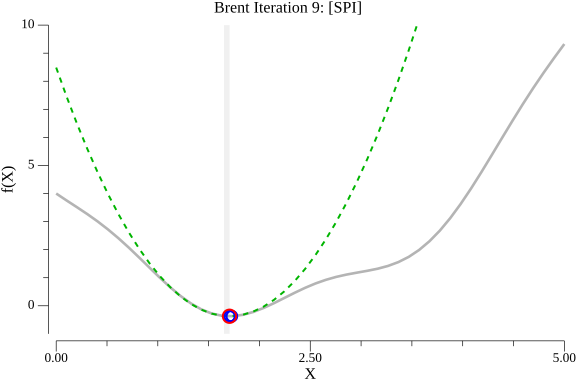
\includegraphics[width=\textwidth]{material/brent/output/brent_09.png}}
      \only<11>{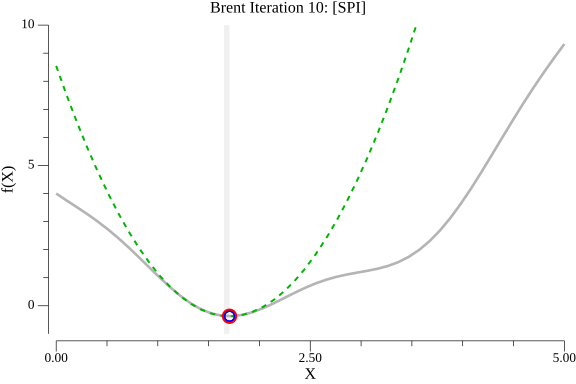
\includegraphics[width=\textwidth]{material/brent/output/brent_10.png}}
      \only<12>{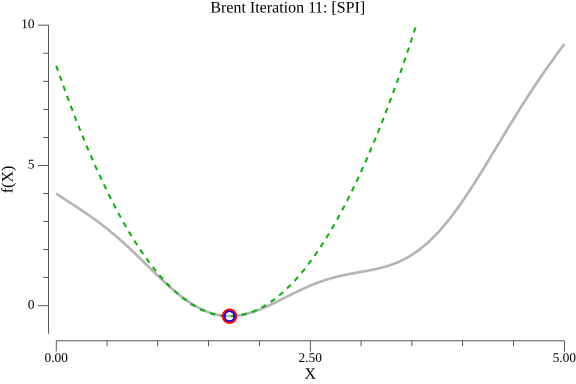
\includegraphics[width=\textwidth]{material/brent/output/brent_11.png}}
      \only<13>{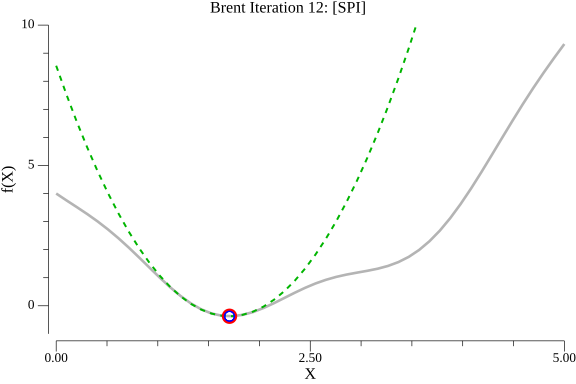
\includegraphics[width=\textwidth]{material/brent/output/brent_12.png}}
    \end{column}
  \end{columns}
\end{frame}
 % ハイブリット手法としてBrent法を紹介
%===========================================================
% 4. 応用例：最良近似多項式の計算
%===========================================================
\section{応用例}


% 比較スライド (1/3: テーブル)
\begin{frame}{黄金分割法とBrent法の比較}
  \begin{table}
    \centering
    \caption{収束性能の比較 (誤差 $10^{-8}$ 到達まで)}
    \begin{tabular}{|l|r|r|r|} \hline
      \textbf{手法} & \textbf{イテレーション} & \textbf{計算時間 (ms)} & \textbf{収束次数} \\ \hline \hline
      黄金分割法 & 42回 & 0.0093 & 1.000 \\
      \textbf{Brent法} & \textbf{16回} & \textbf{0.0029} & $\approx 1.324$ \\ \hline
      \textbf{Golden/Brent} & \textbf{2.62×} & \textbf{3.21×} & - \\ \hline
    \end{tabular}
  \end{table}

  \vspace{1em}

  \begin{itemize}
    \item Brent法は黄金分割法と比べ、\textbf{イテレーション数で約 2.6倍高速}に収束
    \item さらに、\textbf{計算時間では約 3.21倍高速}に収束
    \item Brent法の放物線補間が効率的に機能していることを示す
    \item \href{run:code brent_iterations.txt}{\textcolor{blue}{両手法の変数推移表を参照}}
  \end{itemize}
\end{frame}

% 比較スライド (2/3: グラフ)
\begin{frame}{黄金分割法とBrent法の比較：収束履歴}
  \begin{figure}
    \centering
    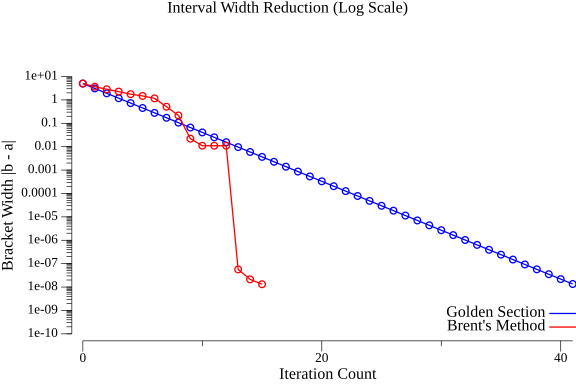
\includegraphics[width=0.75\textwidth]{material/full/output/width_plot.png}
    \caption{区間幅の縮小}
  \end{figure}
\end{frame}

% 比較スライド (3/3: 考察)
\begin{frame}{収束性能の考察}
  \begin{itemize}
    \item 黄金分割法は対数軸で直線的に減衰（線形収束）
    \item Brent法は放物線補間が効き始めると急激に減衰（超線形収束）
    \vspace{1em}
    \item \textbf{結論}:
    \begin{itemize}
      \item Brent法は黄金分割法と比べ、イテレーション数で約 2.6倍高速に収束
      \item 計算時間では約 3.21倍高速に収束
      \item 放物線補間が効率的に機能していることを示す
    \end{itemize}
  \end{itemize}
\end{frame}
 % 黄金分割法 VS Brent法

\end{document}